%% LyX 2.3.7 created this file.  For more info, see http://www.lyx.org/.
%% Do not edit unless you really know what you are doing.
\documentclass[journal,article,submit,pdftex,moreauthors]{mdpi}
\usepackage[utf8]{inputenc}
\usepackage{float}
\usepackage{url}
\usepackage{amsmath}
\usepackage{graphicx}

\makeatletter

%%%%%%%%%%%%%%%%%%%%%%%%%%%%%% LyX specific LaTeX commands.

\Title{Constructing the bounds for neural network training using Grammatical
Evolution}

\TitleCitation{Constructing the bounds for neural network training using Grammatical
Evolution}

\newcommand{\orcidauthorA}{0000-0000-0000-000X}


\newcommand{\orcidauthorB}{0000-0000-0000-000X}


\Author{Ioannis G. Tsoulos$^{1,\dagger,*}$, Alexandros Tzallas$^{2,\dagger}$,
Evangelos Karvounis $^{3}$}

\AuthorNames{Ioannis G. Tsoulos, Alexandros Tzallas and Evangelos Karvounis }

\AuthorCitation{Tsoulos, I,G.; Tzallas, A.; Karvounis, E. }


\address{$^{1}$\quad{}Department of Informatics and Telecommunications,
University of Ioannina, Greece; itsoulos@uoi.gr\\
$^{2}$\quad{}Department of Informatics and Telecommunications, University
of Ioannina, Greece; tzallas@uoi.gr\\
$^{3}\quad$Department of Informatics and Telecommunications, University
of Ioannina, Greece; ekarvounis@uoi.gr}


\corres{Correspondence: itsoulos@uoi.gr;}


\firstnote{Current address: Department of Informatics and Telecommunications,
University of Ioannina, Greece.}


\secondnote{These authors contributed equally to this work.}


\abstract{Artificial neural networks are widely established models of computational
intelligence that have been tested for effectiveness in a variety
of real-world applications. These models require fitting a set of
parameters through the use of some optimization technique. However,
an issue that researchers often face is finding an efficient range
of values for the parameters of the artificial neural network. This
paper proposes an innovative technique of generating a promising range
of values for the parameters of the artificial neural network. Finding
the value field is done by a series of rules for partitioning the
original set of values or expanding it, which rules are generated
using Grammatical Evolution. After finding a promising interval of
values, any optimization technique such as a genetic algorithm can
be used to train the artificial neural network on that interval of
values. The new technique was tested on a wide range of problems from
the relevant literature and the results were extremely promising.}


\keyword{Neural networks; Genetic algorithms; Grammatical Evolution}

\DeclareTextSymbolDefault{\textquotedbl}{T1}
%% Because html converters don't know tabularnewline
\providecommand{\tabularnewline}{\\}

%%%%%%%%%%%%%%%%%%%%%%%%%%%%%% Textclass specific LaTeX commands.
\newenvironment{lyxcode}
	{\par\begin{list}{}{
		\setlength{\rightmargin}{\leftmargin}
		\setlength{\listparindent}{0pt}% needed for AMS classes
		\raggedright
		\setlength{\itemsep}{0pt}
		\setlength{\parsep}{0pt}
		\normalfont\ttfamily}%
	 \item[]}
	{\end{list}}

%%%%%%%%%%%%%%%%%%%%%%%%%%%%%% User specified LaTeX commands.
%  LaTeX support: latex@mdpi.com 
%  For support, please attach all files needed for compiling as well as the log file, and specify your operating system, LaTeX version, and LaTeX editor.

%=================================================================


% For posting an early version of this manuscript as a preprint, you may use "preprints" as the journal and change "submit" to "accept". The document class line would be, e.g., \documentclass[preprints,article,accept,moreauthors,pdftex]{mdpi}. This is especially recommended for submission to arXiv, where line numbers should be removed before posting. For preprints.org, the editorial staff will make this change immediately prior to posting.

%--------------------
% Class Options:
%--------------------
%----------
% journal
%----------
% Choose between the following MDPI journals:
% acoustics, actuators, addictions, admsci, adolescents, aerospace, agriculture, agriengineering, agronomy, ai, algorithms, allergies, alloys, analytica, animals, antibiotics, antibodies, antioxidants, applbiosci, appliedchem, appliedmath, applmech, applmicrobiol, applnano, applsci, aquacj, architecture, arts, asc, asi, astronomy, atmosphere, atoms, audiolres, automation, axioms, bacteria, batteries, bdcc, behavsci, beverages, biochem, bioengineering, biologics, biology, biomass, biomechanics, biomed, biomedicines, biomedinformatics, biomimetics, biomolecules, biophysica, biosensors, biotech, birds, bloods, blsf, brainsci, breath, buildings, businesses, cancers, carbon, cardiogenetics, catalysts, cells, ceramics, challenges, chemengineering, chemistry, chemosensors, chemproc, children, chips, cimb, civileng, cleantechnol, climate, clinpract, clockssleep, cmd, coasts, coatings, colloids, colorants, commodities, compounds, computation, computers, condensedmatter, conservation, constrmater, cosmetics, covid, crops, cryptography, crystals, csmf, ctn, curroncol, currophthalmol, cyber, dairy, data, dentistry, dermato, dermatopathology, designs, diabetology, diagnostics, dietetics, digital, disabilities, diseases, diversity, dna, drones, dynamics, earth, ebj, ecologies, econometrics, economies, education, ejihpe, electricity, electrochem, electronicmat, electronics, encyclopedia, endocrines, energies, eng, engproc, ent, entomology, entropy, environments, environsciproc, epidemiologia, epigenomes, est, fermentation, fibers, fintech, fire, fishes, fluids, foods, forecasting, forensicsci, forests, foundations, fractalfract, fuels, futureinternet, futureparasites, futurepharmacol, futurephys, futuretransp, galaxies, games, gases, gastroent, gastrointestdisord, gels, genealogy, genes, geographies, geohazards, geomatics, geosciences, geotechnics, geriatrics, hazardousmatters, healthcare, hearts, hemato, heritage, highthroughput, histories, horticulturae, humanities, humans, hydrobiology, hydrogen, hydrology, hygiene, idr, ijerph, ijfs, ijgi, ijms, ijns, ijtm, ijtpp, immuno, informatics, information, infrastructures, inorganics, insects, instruments, inventions, iot, j, jal, jcdd, jcm, jcp, jcs, jdb, jeta, jfb, jfmk, jimaging, jintelligence, jlpea, jmmp, jmp, jmse, jne, jnt, jof, joitmc, jor, journalmedia, jox, jpm, jrfm, jsan, jtaer, jzbg, kidney, kidneydial, knowledge, land, languages, laws, life, liquids, literature, livers, logics, logistics, lubricants, lymphatics, machines, macromol, magnetism, magnetochemistry, make, marinedrugs, materials, materproc, mathematics, mca, measurements, medicina, medicines, medsci, membranes, merits, metabolites, metals, meteorology, methane, metrology, micro, microarrays, microbiolres, micromachines, microorganisms, microplastics, minerals, mining, modelling, molbank, molecules, mps, msf, mti, muscles, nanoenergyadv, nanomanufacturing, nanomaterials, ncrna, network, neuroglia, neurolint, neurosci, nitrogen, notspecified, nri, nursrep, nutraceuticals, nutrients, obesities, oceans, ohbm, onco, oncopathology, optics, oral, organics, organoids, osteology, oxygen, parasites, parasitologia, particles, pathogens, pathophysiology, pediatrrep, pharmaceuticals, pharmaceutics, pharmacoepidemiology, pharmacy, philosophies, photochem, photonics, phycology, physchem, physics, physiologia, plants, plasma, pollutants, polymers, polysaccharides, poultry, powders, preprints, proceedings, processes, prosthesis, proteomes, psf, psych, psychiatryint, psychoactives, publications, quantumrep, quaternary, qubs, radiation, reactions, recycling, regeneration, religions, remotesensing, reports, reprodmed, resources, rheumato, risks, robotics, ruminants, safety, sci, scipharm, seeds, sensors, separations, sexes, signals, sinusitis, skins, smartcities, sna, societies, socsci, software, soilsystems, solar, solids, sports, standards, stats, stresses, surfaces, surgeries, suschem, sustainability, symmetry, synbio, systems, taxonomy, technologies, telecom, test, textiles, thalassrep, thermo, tomography, tourismhosp, toxics, toxins, transplantology, transportation, traumacare, traumas, tropicalmed, universe, urbansci, uro, vaccines, vehicles, venereology, vetsci, vibration, viruses, vision, waste, water, wem, wevj, wind, women, world, youth, zoonoticdis 

%---------
% article
%---------
% The default type of manuscript is "article", but can be replaced by: 
% abstract, addendum, article, book, bookreview, briefreport, casereport, comment, commentary, communication, conferenceproceedings, correction, conferencereport, entry, expressionofconcern, extendedabstract, datadescriptor, editorial, essay, erratum, hypothesis, interestingimage, obituary, opinion, projectreport, reply, retraction, review, perspective, protocol, shortnote, studyprotocol, systematicreview, supfile, technicalnote, viewpoint, guidelines, registeredreport, tutorial
% supfile = supplementary materials

%----------
% submit
%----------
% The class option "submit" will be changed to "accept" by the Editorial Office when the paper is accepted. This will only make changes to the frontpage (e.g., the logo of the journal will get visible), the headings, and the copyright information. Also, line numbering will be removed. Journal info and pagination for accepted papers will also be assigned by the Editorial Office.

%------------------
% moreauthors
%------------------
% If there is only one author the class option oneauthor should be used. Otherwise use the class option moreauthors.

%---------
% pdftex
%---------
% The option pdftex is for use with pdfLaTeX. If eps figures are used, remove the option pdftex and use LaTeX and dvi2pdf.

%=================================================================
% MDPI internal commands - do not modify
\firstpage{1} 
 
\setcounter{page}{\@firstpage} 

\pubvolume{1}
\issuenum{1}
\articlenumber{0}
\pubyear{2023}
\copyrightyear{2023}
%\externaleditor{Academic Editor: Firstname Lastname} % For journal Automation, please change Academic Editor to "Communicated by"
\datereceived{}
\daterevised{ } % Comment out if no revised date
\dateaccepted{}
\datepublished{}
%\datecorrected{} % Corrected papers include a "Corrected: XXX" date in the original paper.
%\dateretracted{} % Corrected papers include a "Retracted: XXX" date in the original paper.
\hreflink{https://doi.org/} % If needed use \linebreak
%\doinum{}
%------------------------------------------------------------------
% The following line should be uncommented if the LaTeX file is uploaded to arXiv.org
%\pdfoutput=1

%=================================================================
% Add packages and commands here. The following packages are loaded in our class file: fontenc, inputenc, calc, indentfirst, fancyhdr, graphicx, epstopdf, lastpage, ifthen, lineno, float, amsmath, setspace, enumitem, mathpazo, booktabs, titlesec, etoolbox, tabto, xcolor, soul, multirow, microtype, tikz, totcount, changepage, attrib, upgreek, cleveref, amsthm, hyphenat, natbib, hyperref, footmisc, url, geometry, newfloat, caption

%=================================================================
%% Please use the following mathematics environments: Theorem, Lemma, Corollary, Proposition, Characterization, Property, Problem, Example, ExamplesandDefinitions, Hypothesis, Remark, Definition, Notation, Assumption
%% For proofs, please use the proof environment (the amsthm package is loaded by the MDPI class).

%=================================================================
% The fields PACS, MSC, and JEL may be left empty or commented out if not applicable
%\PACS{J0101}
%\MSC{}
%\JEL{}

%%%%%%%%%%%%%%%%%%%%%%%%%%%%%%%%%%%%%%%%%%
% Only for the journal Diversity
%\LSID{\url{http://}}

%%%%%%%%%%%%%%%%%%%%%%%%%%%%%%%%%%%%%%%%%%
% Only for the journal Applied Sciences:
%\featuredapplication{Authors are encouraged to provide a concise description of the specific application or a potential application of the work. This section is not mandatory.}
%%%%%%%%%%%%%%%%%%%%%%%%%%%%%%%%%%%%%%%%%%

%%%%%%%%%%%%%%%%%%%%%%%%%%%%%%%%%%%%%%%%%%
% Only for the journal Data:
%\dataset{DOI number or link to the deposited data set in cases where the data set is published or set to be published separately. If the data set is submitted and will be published as a supplement to this paper in the journal Data, this field will be filled by the editors of the journal. In this case, please make sure to submit the data set as a supplement when entering your manuscript into our manuscript editorial system.}

%\datasetlicense{license under which the data set is made available (CC0, CC-BY, CC-BY-SA, CC-BY-NC, etc.)}

%%%%%%%%%%%%%%%%%%%%%%%%%%%%%%%%%%%%%%%%%%
% Only for the journal Toxins
%\keycontribution{The breakthroughs or highlights of the manuscript. Authors can write one or two sentences to describe the most important part of the paper.}

%%%%%%%%%%%%%%%%%%%%%%%%%%%%%%%%%%%%%%%%%%
% Only for the journal Encyclopedia
%\encyclopediadef{Instead of the abstract}
%\entrylink{The Link to this entry published on the encyclopedia platform.}
%%%%%%%%%%%%%%%%%%%%%%%%%%%%%%%%%%%%%%%%%%

%%%%%%%%%%%%%%%%%%%%%%%%%%%%%%%%%%%%%%%%%%
% Only for the journal Advances in Respiratory Medicine
%\addhighlights{yes}
%\renewcommand{\addhighlights}{%

%\noindent This is an obligatory section in “Advances in Respiratory Medicine”, whose goal is to increase the discoverability and readability of the article via search engines and other scholars. Highlights should not be a copy of the abstract, but a simple text allowing the reader to quickly and simplified find out what the article is about and what can be cited from it. Each of these parts should be devoted up to 2~bullet points.\vspace{3pt}\\
%\textbf{What are the main findings?}
% \begin{itemize}[labelsep=2.5mm,topsep=-3pt]
% \item First bullet.
% \item Second bullet.
% \end{itemize}\vspace{3pt}
%\textbf{What is the implication of the main finding?}
% \begin{itemize}[labelsep=2.5mm,topsep=-3pt]
% \item First bullet.
% \item Second bullet.
% \end{itemize}
%}
%%%%%%%%%%%%%%%%%%%%%%%%%%%%%%%%%%%%%%%%%%

\makeatother

\begin{document}
\maketitle

\section{Introduction}

Artificial neural networks (ANNs) are widespread machine learning
models, which base their dynamics on a series of parameters which
are also called computational units or weights in the relevant literature\citep{nn1,nn2}.
Neural networks are widely used in a variety of scientific applications,
such as problems from physics \citep{nnphysics1,nnphysics2,nnphysics3},
solutions of differential equations \citep{nnde1,nnde2}, agriculture
problems \citep{nnagr1,nnagr2}, chemistry problems \citep{nnchem1,nnchem2,nnchem3},
problems that appear in the area of economic sciences \citep{nnecon1,nnecon2,nncecon3},
problems related to medicine \citep{nnmed1,nnmed2} etc. Commonly,
the neural networks are expressed as a function $N(\overrightarrow{x},\overrightarrow{w})$,
with the assumption that the vector $\overrightarrow{x}$ stands for
the input vector to the neural network and the vector $\overrightarrow{w}$
is the parameter vector that should be estimated. The first vector
is called pattern in the bibliography and the second one weight vector.
Techniques that adjust the parameter vector $\overrightarrow{w}$
minimize the so-called training error, defined as:
\begin{equation}
E\left(N\left(\overrightarrow{x},\overrightarrow{w}\right)\right)=\sum_{i=1}^{M}\left(N\left(\overrightarrow{x}_{i},\overrightarrow{w}\right)-y_{i}\right)^{2}\label{eq:eq1}
\end{equation}
In equation \ref{eq:eq1} the set $\left(\overrightarrow{x_{i}},y_{i}\right),\ i=1,...,M$
is denoted as the train set of the neural network. The $y_{i}$ are
considered the target outputs for the $\overrightarrow{x_{i}}$ points
. As proposed in \citep{nnc}, neural networks can be expressed as
the following summation:
\begin{equation}
N\left(\overrightarrow{x},\overrightarrow{w}\right)=\sum_{i=1}^{H}w_{(d+2)i-(d+1)}\sigma\left(\sum_{j=1}^{d}x_{j}w_{(d+2)i-(d+1)+j}+w_{(d+2)i}\right)\label{eq:nn}
\end{equation}
The number of processing units is denoted by $H$ and the value $d$
stands for the dimension of input vector $\overrightarrow{x}$. The
function$\ \sigma(x)$ denotes the well - known sigmoid function expressed
as: 
\begin{equation}
\sigma(x)=\frac{1}{1+\exp(-x)}\label{eq:sig}
\end{equation}
From the above equations one can calculated the total number of parameters
in the neural network as:
\begin{equation}
n=\left(d+2\right)H
\end{equation}
The training of neural networks has been performed by a variety of
numerical methods in recent bibliography, such as: the Back Propagation
method \citep{bpnn,bpnn2}, the RPROP method \citep{rpropnn-1,rpropnn2,rpropnn3},
the Adam optimizer \citep{Adam,AdamNN} etc. Furthermore, more advanced
optimization methods have been incorporated to optimize the parameter
vector of neural networks by minimizing equation \ref{eq:eq1} such
as Quasi Newton methods \citep{quasinn,quasinn2},\textbf{ }the Tabu
Search method \citep{tabunn}, Simulated Annealing \citep{nn_ann1,nn_ann2},
Genetic Algorithms \citep{geneticnn,geneticnn2}, Particle Swarm Optimization
\citep{psonn,psonn2},\textbf{ }Differential Evolution \citep{weight_de1,weight_de2},
Ant Colony Optimization \citep{weight_aco} etc. 

Also, recently a series of hybrid optimization methods have been proposed
to tackle the minimization of the training error, such as a method
that combines PSO and genetic algorithms \citep{nnhybrid1,nnhybrid2},
incorporation of a particle swarm optimization algorithm and gravitational
search algorithm \citep{nnhybrid3}, a combination of a genetic algorithm
and controlled gradient method \citep{nnhybrid4} etc.

In addition, an important topic for artificial neural networks such
as parameter initialization has been studied by several researchers
in recent years. In this area appeared papers such as initialization
with decision trees \citep{weight_init1}, incorporation of the Cauchy's
inequality \citep{weight_init2}, discriminant learning \citep{weight_init3}
etc. Also, another interesting topic in the area of neural networks
is weight decaying, where some regularization is applied to the parameters
of the neural network to avoid the overfitting problem. For this topic,
several research papers have been suggested, such as a method that
incorporates positive correlation \citep{weight_decay1}, the SarProp
algorithm \citep{weight_decay2}, usage of pruning techniques \citep{weight_decay3}
etc.

This paper proposes a two-stage method for efficient training of the
parameters of artificial neural networks. In the first stage, a value
interval is constructed for the parameters of the neural network through
Grammatical Evolution \citep{ge1}. In the first stage of this work,
after an initial estimate of the interval for the parameters of the
neural network is made, a series of rules for partitioning and expanding
the initial value interval are applied with the usage of Grammatical
Evolution, until a promising value interval is found. In the second
stage of the method, a genetic algorithm is applied to train the parameters
of the artificial neural network. Training is performed within the
optimal interval of values found in the first stage of the method.

The rest of this article is organized as follows: in section \ref{sec:Method-description}
the steps of the proposed method are outlined in detail, in section
\ref{sec:Experiments} the datasets used in the conducted experiments
as well the experimental results are presented and finally in section
\ref{sec:Conclusions} some conclusions are presented.

\section{Method description\label{sec:Method-description}}

In this section a detailed description of the Grammatical Evolution
technique is provided, accompanied by the proposed language that creates
intervals for the parameters of the neural networks.\textbf{ }Subsequently\textbf{,}
the first phase of the proposed technique is described and finally,
the second phase with the application of a Genetic Algorithm to the
outcome of the first phase, is thoroughly analyzed.

\subsection{Grammatical evolution }

Grammatical evolution is an evolutionary process, where the chromosomes
represent production rules of some provided BNF (Backus--Naur form)
grammar\citep{bnf1} and this\textbf{ }evolutionary process can evolve
programs in the underlying language. Grammatical Evolution has been
used successfully in many real world problems, such as function approximation\citep{ge_program1,ge_program2},
solution of trigonometric equations \citep{ge_trig}, automatic music
composition \citep{ge_music}, neural network construction \citep{ge_nn,ge_nn2},
creating numeric constraints\citep{ge_constant}, video games \citep{ge_pacman,ge_supermario},
estimation of energy demand\citep{ge_energy}, combinatorial optimization
\citep{ge_comb}, cryptography \citep{ge_crypt}, evolution of decision
trees \citep{ge_decision}, automatic design of analog electronic
circuits \citep{ge_analog} etc\textbf{. }Any BNF grammar can be described
as the set $G=\left(N,T,S,P\right)$ where
\begin{itemize}
\item $N$ is the set of the non-terminal symbols. Every symbol in $N$
has a series of production rules, used to produce terminal symbols.
\item \textbf{$T$ }is the set of terminal symbols. 
\item $S$ denotes the start symbol of the grammar, with $S\in N$.
\item $P$ is the set of production rules, to create terminal symbols non
- terminal symbols. These rules are in the form $A\rightarrow a$
or $A\rightarrow aB,\ A,B\in N,\ a\in T$.
\end{itemize}
The algorithm initiates from the symbol $S$ and iteratively produces
terminal symbols by replacing non-terminal symbols with the right
hand of the selected production rule. Every production rule is is
selected using the following steps:
\begin{itemize}
\item Get the next element V from the current chromosome.
\item Select the next production rule according to: Rule = V mod $N_{R}$,
where $N_{R}$ is the total number of production rules for the current
non -- terminal symbol. 
\end{itemize}
The grammar used in the current work is shown in Figure \ref{fig:BNF-grammar-of}.

\begin{figure}[H]
\caption{BNF grammar used in the current work. The value $n$ stands for the
number of total parameters in the neural network.\label{fig:BNF-grammar-of}}

\begin{lyxcode}
S::=\textless expr\textgreater ~~~(0)~

\textless expr\textgreater ~::=~~(\textless xlist\textgreater ~,~\textless lcommand\textgreater ,\textless rcommand\textgreater )~~(0)~~~~~~~~~~~~~

~~~~~~~~~~~\textbar\textless expr\textgreater ,\textless expr\textgreater ~~~~~~~~~~~~~~~~(1)

\textless xlist\textgreater ::=x1~~~~(0)~~~~~~~~~~~~~~

~~~~~~~~~~~\textbar ~x2~(1)~~~~~~~~~~~~~~

~~~~~~~~~~~………~~~~~~~~~~~~~

~~~~~~~~~~~\textbar ~xn~(n)

\textless left\_command\textgreater ~~::=~NOTHING~(0)~~~~~~~~~~~~~

~~~~~~~~~~~\textbar ~~~~~~~~EXPAND~~(1)

~~~~~~~~~~~\textbar ~~~~~~~~DIVIDE~~(2)

\textless right\_command\textgreater ~::=~NOTHING~(0)

~~~~~~~~~~~\textbar ~~~~~~~~EXPAND~~(1)

~~~~~~~~~~~\textbar ~~~~~~~~DIVIDE~~(2)
\end{lyxcode}
\end{figure}
The symbols in \textless\textgreater{} represent the non-terminal
symbols of the grammar. The numbers in parentheses in the right part
of each rule, indicate production rule sequence numbers. In the proposed
language described by the grammar of the scheme, three distinct operations
can be applied to parameters of the artificial neural network either
on the left end of the parameter's value range (described by \textless lcommand\textgreater )
or on the right end of the value range (described by the \textless rcommand\textgreater{}
symbol). These commands are
\begin{enumerate}
\item NOTHING. This command means that no action takes place.
\item EXPAND. With this command, the corresponding end of the value field
is extended by 50\% of the width of the field.
\item DIVIDE. With this command, the corresponding end of the value field
is shrunk by 50\% of the width of the field.
\end{enumerate}
As a complete example consider a neural network with $H=2$ hidden
nodes and the dimension of the objective problem is set to $d=2$.
Hence, the total number of parameters in the neural network is $n=(d+2)H=8$.
Also, for reasons of simplicity, we consider that the initial range
of values for all parameters of the artificial neural network is the
interval {[}-2,2{]} and is denotes as a the set of intervals
\begin{equation}
I_{N}=\left\{ \left[-2,2\right],\left[-2,2\right],\left[-2,2\right],\left[-2,2\right],\left[-2,2\right],\left[-2,2\right],\left[-2,2\right],\left[-2,2\right]\right\} \label{eq:in_original}
\end{equation}
 and consider also the chromosome 
\[
x=\left[9,8,6,4,15,9,16,23,7\right]
\]
 The steps to produce the final program 
\[
p_{\mbox{test}}=(x7,\mbox{EXPAND},\mbox{NOTHING}),(x1,\mbox{DIVIDE},\mbox{EXPAND})
\]
 are shown in Table \ref{tab:table_with_steps}. 

\begin{table}[H]
\caption{Steps to produce a valid expression from the BNF grammar.\label{tab:table_with_steps}}

\centering{}%
\begin{tabular}{|c|c|c|}
\hline 
Expression & Chromosome & Operation\tabularnewline
\hline 
\hline 
 & 9,8,6,4,15,9,16,23,8 & 9 mod 2=1\tabularnewline
\hline 
{\footnotesize{}\textless expr\textgreater ,\textless expr\textgreater} & 8,6,4,15,9,16,23,8 & 8 mod 2=0\tabularnewline
\hline 
{\footnotesize{}(\textless xlist\textgreater ,\textless lcommand\textgreater ,\textless rcommand\textgreater ),\textless expr\textgreater} & 6,4,15,9,16,23,8 & 6 mod 8=6\tabularnewline
\hline 
{\footnotesize{}(x7,\textless lcommand\textgreater ,\textless rcommand\textgreater ),\textless expr\textgreater} & 4,15,9,16,23,8 & 4 \% 3=1\tabularnewline
\hline 
{\footnotesize{}(x7,EXPAND,\textless rcommand\textgreater ),\textless expr\textgreater} & 15,9,16,23,8 & 15\%3=0\tabularnewline
\hline 
{\footnotesize{}(x7,EXPAND,NOTHING),\textless expr\textgreater} & 9,16,23,8 & 9 \%2 =1\tabularnewline
\hline 
{\footnotesize{}(x7,EXPAND,NOTHING),(\textless xlist\textgreater ,\textless lcommand\textgreater ,\textless rcommand\textgreater )} & 16,23,8 & 16\%8=0\tabularnewline
\hline 
{\footnotesize{}(x7,EXPAND,NOTHING),(x1,\textless lcommand\textgreater ,\textless rcommand\textgreater )} & 23,8 & 23\%3=2\tabularnewline
\hline 
{\footnotesize{}(x7,EXPAND,NOTHING),(x1,DIVIDE,\textless rcommand\textgreater )} & 8 & 8\%3=2\tabularnewline
\hline 
{\footnotesize{}(x7,EXPAND,NOTHING),(x1,DIVIDE,EXPAND)} &  & \tabularnewline
\hline 
\end{tabular}
\end{table}
After the application of the program $p_{\mbox{test}}$ to the original
interval $I_{N}$ of equation \ref{eq:in_original}, the new set has
as follows:
\begin{equation}
I_{N}=\left\{ \left[-4,2\right],\left[-2,2\right],\left[-2,2\right],\left[-2,2\right],\left[-2,2\right],\left[-2,2\right],\left[0,4\right],\left[-2,2\right]\right\} 
\end{equation}


\subsection{The first phase of the proposed method \label{subsec:The-first-phase}}

Before starting the process of creating partitioning rules and expanding
the value interval of the neural network weights, an initial estimate
of this interval should be made. In the present work, only a few steps
of a genetic algorithm are applied to make an initial estimate of
the value interval. At the end of the genetic algorithm, the chromosome
with the best value is the 
\begin{equation}
\mbox{IX}=\left(\mbox{IX}_{1},\mbox{IX}_{2},\ldots,\mbox{IX}_{n}\right)
\end{equation}
So, the initial interval set for the parameters of the neural network
is calculated as
\begin{equation}
I_{N}=\left\{ \left[-\mbox{IX}_{1},\mbox{IX}_{1}\right],\left\{ -\mbox{IX}_{2},\mbox{IX}_{2}\right\} ,\ldots,\left[-\mbox{IX}_{n},\mbox{IX}_{n}\right]\right\} 
\end{equation}
The first phase of the proposed technique will accept the set $I_{N}$
as input and seek to compute a new set by reducing the training error
of the artificial neural network. The first step is mainly a genetic
algorithm and the corresponding steps are as follows:
\begin{enumerate}
\item \textbf{Set} $N_{c}$ as the number of chromosomes for the Grammatical
Evolution.
\item \textbf{Set} as $H$ the number of weights for the neural network.
\item \textbf{Set} $N_{g}$ the maximum number of allowed generations.
\item \textbf{Set} as $p_{s}$ the selection rate , with $p_{s}\le1$.
\item \textbf{Set} as $p_{m}$ the mutation rate, with $p_{m}\le1$.
\item \textbf{Set} $N_{s}$ as the number of randomly created neural networks,
that will be used in the fitness calculation.
\item \textbf{Initialize} randomly the $N_{c}$ chromosomes. Every chromosome
is a set of integer numbers used to produce valid programs through
Grammatical Evolution and the associated grammar of Figure \ref{fig:BNF-grammar-of}.
\item \textbf{Set} $f^{*}=\left[\infty,\infty\right]$, the best discovered
fitness. For this algorithm, we consider the fitness function $f_{g}$
of any given chromosome $g$ as an interval \textbf{$f_{g}=\left[f_{g,\mbox{low}},f_{g,\mbox{upper}}\right]$}
\item \textbf{Set} iter=0. 
\item \textbf{For} $i=1,\ldots,N_{c}$ \textbf{do\label{enu:For--do}}
\begin{enumerate}
\item \textbf{Create }for the chromosome $c_{i}$ the corresponding program
$p_{i}$ using the grammar of Figure \ref{fig:BNF-grammar-of}.
\item \textbf{Apply }the program $p_{i}$ to $I_{N}$ in order to produce
the bounds $\left[\vec{L_{p_{i}}},\overrightarrow{R_{p_{i}}}\right]$. 
\item \textbf{Set} $E_{\mbox{min}}=\infty,\ E_{\mbox{max}}=-\infty$
\item \textbf{For} $j=1,\ldots,N_{S}$ \textbf{do}
\begin{enumerate}
\item \textbf{Create} randomly $g_{j}\in$$\left[\vec{L_{p_{i}}},\overrightarrow{R_{p_{i}}}\right]$
as a set for the parameters of neural network.
\item \textbf{Calculate} the associated training error $E_{g_{j}}=\sum_{k=1}^{M}\left(N\left(\overrightarrow{x}_{k},\overrightarrow{g_{j}}\right)-y_{k}\right)^{2}$
\item \textbf{If} $E_{g_{j}}\le E_{\mbox{min}}$ \textbf{then} $E_{\mbox{min}}=E_{g_{j}}$
\item \textbf{If} $E_{g_{j}}\ge E_{\mbox{max}}$ \textbf{then} $E_{\mbox{max}}=E_{g_{j}}$
\end{enumerate}
\item \textbf{EndFor}
\item \textbf{Set} $f_{i}=\left[E_{\mbox{min}},E_{\mbox{max}}\right]$ as
the fitness value for the chromosome $c_{i}$.
\end{enumerate}
\item \textbf{EndFor }
\item \textbf{Apply} the selection procedure. Firstly, the chromosomes are
sorted with correspondence to their fitness values. Since fitness
is considered an interval, a fitness comparison function is required.
For this reason the operator $L^{*}\left(f_{a},f_{b}\right)$ to compare
two fitness values $f_{a}=\left[a_{1},a_{2}\right]$ and $f_{b}=\left[b_{1},b_{2}\right]$
as follows:
\begin{eqnarray}
L^{*}\left(f_{a},f_{b}\right) & = & \begin{cases}
\mbox{TRUE}, & a_{1}<b_{1},\mbox{OR\ \ensuremath{\left(a_{1}=b_{1}\ \mbox{AND}\ a_{2}<b_{2}\right)}}\\
\mbox{FALSE}, & \mbox{\mbox{OTHERWISE}}
\end{cases}\label{eq:eql}
\end{eqnarray}
In practice this means that the fitness value $f_{a}$ is considered
smaller than $f_{b}$ if $L^{*}\left(f_{a},f_{b}\right)=\mbox{TRUE}$.
The first $\left(1-p_{s}\right)\times N_{c}$ chromosomes with the
lowest fitness values are copied to the next generation. The remaining
chromosomes are substituted by chromosomes produced by the crossover
procedure. During the selection process, for every new offspring,
two chromosomes are selected as parents from the population using
well - known procedure of tournament selection. 
\item \textbf{Apply} the crossover procedure.\textbf{ }For each pair $(z,w)$
of parents, two new chromosomes $\tilde{z}$ and $\tilde{w}$ are
created using the one - point crossover, graphically shown in Figure
\ref{fig:onepoint}.
\item \textbf{Apply} the mutation procedure. For each element of every chromosome
alter the corresponding element with probability $p_{m}$.
\item \textbf{Set} iter=iter+1
\item \textbf{If} $\mbox{iter\ensuremath{\le N_{g}} }$goto step \ref{enu:For--do}.
\end{enumerate}
\begin{figure}[H]
\begin{centering}
\includegraphics[scale=0.5]{onepoint_crossover}
\par\end{centering}
\caption{The one point crossover, used in the Grammatical Evolution.\label{fig:onepoint}}
\end{figure}


\subsection{The second phase of the proposed method}
\begin{enumerate}
\item \textbf{Initialization Step}
\begin{enumerate}
\item \textbf{Set} $N_{c}$ as the number of chromosomes that participate
in the genetic algorithm.
\item \textbf{Set} $N_{g}$ the maximum number of allowed iterations.
\item \textbf{Set} $H$ the number of weights for the neural network.
\item \textbf{Get} the best interval $S$ from the previous step of subsection
\ref{subsec:The-first-phase}.
\item \textbf{Initialize} using uniform distribution the $N_{C}$ chromosomes
in $S$. 
\item \textbf{Set} as $p_{s}$ the selection rate, with $p_{s}\le1$.
\item \textbf{Set} as $p_{m}$ the mutation rate, with $p_{m}\le1$.
\item \textbf{Set} iter=0.
\end{enumerate}
\item \textbf{Fitness calculation Step \label{enu:Fitness-calculation-Step}}
\begin{enumerate}
\item \textbf{For} $i=1,\ldots,N_{g}$ \textbf{do}
\begin{enumerate}
\item \textbf{Calculate} the fitness $f_{i}$ of chromosome $g_{i}$ as
$f_{i}=\sum_{j=1}^{M}\left(N\left(\overrightarrow{x}_{j},\overrightarrow{g_{i}}\right)-y_{j}\right)^{2}$
\end{enumerate}
\item \textbf{EndFor}
\end{enumerate}
\item \textbf{Genetic operations step}
\begin{enumerate}
\item \textbf{Selection procedure.} Initially, the chromosomes are sorted
according to their fitness values. The first $\left(1-p_{s}\right)\times N_{c}$
chromosomes with the lowest fitness values are copied to the next
generation. The remaining chromosomes are substituted by chromosomes
produced by the crossover procedure. During the selection process,
for every new offspring, two chromosomes are selected as parents from
the population using well - known procedure of tournament selection. 
\item \textbf{Crossover procedure}: For each pair $(z,w)$ of selected parents,
two chromosomes $\tilde{z}$ and $\tilde{w}$ are constructed using
the following equations:
\begin{eqnarray}
\tilde{z_{i}} & = & a_{i}z_{i}+\left(1-a_{i}\right)w_{i}\nonumber \\
\tilde{w_{i}} & = & a_{i}w_{i}+\left(1-a_{i}\right)z_{i}\label{eq:crossover_ali-1}
\end{eqnarray}
Where $a_{i}$ is random number with the property $a_{i}\in[-0.5,1.5]$
\citep{kaelo}. 
\item \textbf{Mutation procedure}:\textbf{ }For each element of every chromosome
alter the corresponding element with probability $p_{m}$.
\end{enumerate}
\item \textbf{Termination Check Step}
\begin{enumerate}
\item \textbf{Set} $iter=iter+1$ 
\item \textbf{If} $\mbox{iter\ensuremath{\le N_{g}} }$goto step \ref{enu:Fitness-calculation-Step}.
else apply a local search procedure to the best chromosome of the
population. In the current work the BFGS variant of Powell \citep{powell}
was used.
\end{enumerate}
%
\end{enumerate}

\section{Experiments \label{sec:Experiments}}

The effectiveness of the proposed method was evaluated on a series
of classification and regression datasets, used in the relevant literature.
These datasets can be downloaded from the following online databases:
\begin{enumerate}
\item UCI dataset repository, \url{https://archive.ics.uci.edu/ml/index.php}\citep{UCL}
\item Keel repository, \url{https://sci2s.ugr.es/keel/datasets.php}\citep{Keel}.
\item The Statlib URL \url{ftp://lib.stat.cmu.edu/datasets/index.html }.
\end{enumerate}

\subsection{Experimental datasets }

The classification datasets used in this paper are the following:
\begin{enumerate}
\item \textbf{Appendictis} a medical purpose dataset, suggested in \citep{appendicitis}. 
\item \textbf{Australian} dataset \citep{australian}, a dataset related
to credit card transactions.
\item \textbf{Balance} dataset \citep{balance}, related to psychological
states. 
\item \textbf{Cleveland} dataset, which is a medical dataset \citep{cleveland1,cleveland2}.
\item \textbf{Dermatology} dataset \citep{dermatology}, a medical dataset
related to erythemato-squamous diseases. 
\item \textbf{Heart} dataset \citep{heart}, a medical dataset related to
heart diseases.
\item \textbf{Hayes roth} dataset \citep{hayesroth}. 
\item \textbf{HouseVotes} dataset \citep{housevotes}, related to votes
in the U.S. House of Representatives Congressmen. 
\item \textbf{Ionosphere} dataset, used for classification of radar returns
from the ionosphere \citep{ion1,ion2}.
\item \textbf{Liverdisorder} dataset \citep{liver}, a medical dataset related
to liver disorders.
\item \textbf{Mammographic} dataset \citep{mammographic}, used to identify
breast tumors.
\item \textbf{Parkinsons} dataset, a medical dataset related to Parkinson's
disease (PD)\citep{parkinsons}.
\item \textbf{Pima} dataset \citep{pima}, used to detect the presence of
diabetes.
\item \textbf{Popfailures} dataset \citep{popfailures}, a dataset related
to climate measurements.
\item \textbf{Regions2} dataset, medical dataset related to hepatitis C
\citep{regions}. 
\item \textbf{Saheart} dataset \citep{saheart}, a medical dataset related
to heart diseases.
\item \textbf{Segment} dataset \citep{segment}, an image processing dataset.
\item \textbf{Wdbc} dataset \citep{wdbc}, a medical dataset related to
breast tumors. 
\item \textbf{Wine} dataset, used to detect the origin of wines \citep{wine1,wine2}.
\item \textbf{Eeg} datasets, a medical dataset related to EEG measurements
\citep{eeg}. There are 3 different cases from this dataset used here
denoted as Z\_F\_S, ZO\_NF\_S, ZONF\_S.
\item \textbf{Zoo} dataset \citep{zoo}, used to classify animals.
\end{enumerate}
The description of the used regression datasets has as follows:
\begin{enumerate}
\item \textbf{Abalone} dataset \citep{abalone}, used to to predict the
age of abalone from physical measurements. 
\item \textbf{Airfoil }dataset, derived from NASA \citep{airfoil}. 
\item \textbf{Baseball} dataset, used to estimate the salary of baseball
players.
\item \textbf{BK} dataset\citep{Stat}, used to predict the points scored
in a basketball game. 
\item \textbf{BL} dataset, an electrical engineering dataset.
\item \textbf{Concrete} dataset\citep{concrete}. 
\item \textbf{Dee} dataset, used to predict the price of electricity.
\item \textbf{Diabetes} dataset, a medical dataset.
\item \textbf{Housing} dataset, provided in \citep{key23}.
\item \textbf{FA} dataset, used to predict the fit body fat. 
\item \textbf{MB} dataset, available from from Smoothing Methods in Statistics
\citep{key21}. 
\item \textbf{MORTGAGE} dataset, related to Economic data from USA.
\item \textbf{PY }dataset, (Pyrimidines problem)\citep{pydataset}.
\item \textbf{Quake} dataset, used to predict the strength of a earthquakes. 
\item \textbf{Treasure} dataset, related to Economic data from USA.
\item \textbf{Wankara} dataset, a dataset related to weather.
\end{enumerate}

\subsection{Experimental results}

The proposed method was coded in ANSI C++ and the optimization methods
were obtained from the freely available from the OPTIMUS computing
environment, downloaded from \url{https://github.com/itsoulos/OPTIMUS/}(accessed
on 9 September 2023). The results were validated using the 10 - fold
validation technique in all datasets. The experiments were executed
30 times for each dataset\textbf{ }using a different seed for the
random generator each time.\textbf{ }The average classification error
is reported for the case of classification datasets and the average
mean test error for the regression datasets. The machine used in the
experiments was an AMD Ryzen 5950X with 128GB of RAM, running the
Debian Linux operating system. The experimental settings are listed
in the{\tiny{} }Table \ref{tab:Experimental-parameters.}.\textbf{
}The experimental results for the classification datasets are shown
in Table \ref{tab:Experiments-for-classification}, while for the
regression datasets the results are shown in Table \ref{tab:exp2}.
The following applies to the results tables:
\begin{enumerate}
\item A genetic algorithm where the parameters have the values of Table
\ref{tab:Experimental-parameters.} used to train a neural network
with $H$ hidden nodes. The results in the experimental tables are
denoted by the label GENETIC.
\item The Adam optimization method is used to train a neural network with
$H$ hidden nodes. The column ADAM denotes the results for this method.
\item The RPROP method is used to train a neural network with $H$ hidden
nodes. The corresponding results are denoted by RPROP in the relevant
tables.
\item The NEAT method (NeuroEvolution of Augmenting Topologies ) \citep{neat},
where the maximum number of allowed generations is the same as in
the case of the Genetic algorithm. 
\item The proposed method (denoted as PROPOSED) was used with the experimental
settings and are shown in Table \ref{tab:Experimental-parameters.}.
\item An extra line was also added to the experimental tables under the
title AVERAGE. This line represents the average classification or
regression error for all datasets.
\end{enumerate}
\begin{table}[H]
\caption{Experimental parameters.\label{tab:Experimental-parameters.}}

\centering{}%
\begin{tabular}{|c|c|}
\hline 
PARAMETER & VALUE\tabularnewline
\hline 
\hline 
$H$ & 10\tabularnewline
\hline 
$N_{C}$ & 200\tabularnewline
\hline 
$N_{S}$ & 50\tabularnewline
\hline 
$N_{t}$ & 200\tabularnewline
\hline 
$p_{s}$ & 0.10\tabularnewline
\hline 
$p_{m}$ & 0.01\tabularnewline
\hline 
\end{tabular}
\end{table}
\begin{table}[H]
\caption{Experiments for classification datasets\label{tab:Experiments-for-classification}}

\centering{}%
\begin{tabular}{|c|c|c|c|c|c|}
\hline 
DATASET & GENETIC & ADAM & RPROP & NEAT & PROPOSED\tabularnewline
\hline 
\hline 
Appendicitis & 18.10\% & 16.50\% & 16.30\% & 17.20\% & 17.00\%\tabularnewline
\hline 
Australian & 32.21\% & 35.65\% & 36.12\% & 31.98\% & 24.55\%\tabularnewline
\hline 
Balance & 8.97\% & 7.87\% & 8.81\% & 23.14\% & 16.71\%\tabularnewline
\hline 
Cleveland & 51.60\% & 67.55\% & 61.41\% & 53.44\% & 47.91\%\tabularnewline
\hline 
Dermatology & 30.58\% & 26.14\% & 15.12\% & 32.43\% & 8.93\%\tabularnewline
\hline 
Hayes Roth & 56.18\% & 59.70\% & 37.46\% & 50.15\% & 32.21\%\tabularnewline
\hline 
Heart & 28.34\% & 38.53\% & 30.51\% & 39.27\% & 17.40\%\tabularnewline
\hline 
HouseVotes & 6.62\% & 7.48\% & 6.04\% & 10.89\% & 3.48\%\tabularnewline
\hline 
Ionosphere & 15.14\% & 16.64\% & 13.65\% & 19.67\% & 7.14\%\tabularnewline
\hline 
Liverdisorder & 31.11\% & 41.53\% & 40.26\% & 30.67\% & 28.90\%\tabularnewline
\hline 
Lymography & 23.26\% & 29.26\% & 24.67\% & 33.70\% & 17.86\%\tabularnewline
\hline 
Mammographic & 19.88\% & 46.25\% & 18.46\% & 22.85\% & 17.32\%\tabularnewline
\hline 
Parkinsons & 18.05\% & 24.06\% & 22.28\% & 18.56\% & 14.35\%\tabularnewline
\hline 
Pima & 32.19\% & 34.85\% & 34.27\% & 34.51\% & 25.58\%\tabularnewline
\hline 
Popfailures & 5.94\% & 5.18\% & 4.81\% & 7.05\% & 4.58\%\tabularnewline
\hline 
Regions2 & 29.39\% & 29.85\% & 27.53\% & 33.23\% & 28.32\%\tabularnewline
\hline 
Saheart & 34.86\% & 34.04\% & 34.90\% & 34.51\% & 27.43\%\tabularnewline
\hline 
Segment & 57.72\% & 49.75\% & 52.14\% & 66.72\% & 20.68\%\tabularnewline
\hline 
Wdbc & 8.56\% & 35.35\% & 21.57\% & 12.88\% & 5.23\%\tabularnewline
\hline 
Wine & 19.20\% & 29.40\% & 30.73\% & 25.43\% & 5.35\%\tabularnewline
\hline 
Z\_F\_S & 10.73\% & 47.81\% & 29.28\% & 38.41\% & 6.56\%\tabularnewline
\hline 
ZO\_NF\_S & 8.41\% & 47.43\% & 6.43\% & 43.75\% & 3.60\%\tabularnewline
\hline 
ZONF\_S & 2.60\% & 11.99\% & 27.27\% & 5.44\% & 2.21\%\tabularnewline
\hline 
ZOO & 16.67\% & 14.13\% & 15.47\% & 20.27\% & 6.10\%\tabularnewline
\hline 
\textbf{AVERAGE} & \textbf{23.60\%} & \textbf{31.54\%} & \textbf{25.65\%} & \textbf{29.42\%} & \textbf{16.23\%}\tabularnewline
\hline 
\end{tabular}
\end{table}
\begin{table}[H]
\caption{Experiments for regression datasets.\label{tab:exp2}}

\centering{}%
\begin{tabular}{|c|c|c|c|c|c|}
\hline 
DATASET & GENETIC & ADAM & RPROP & NEAT & PROPOSED\tabularnewline
\hline 
\hline 
ABALONE & 7.17 & 4.30 & 4.55 & 9.88 & 4.48\tabularnewline
\hline 
AIRFOIL & 0.003 & 0.005 & 0.002 & 0.067 & 0.002\tabularnewline
\hline 
BASEBALL & 103.60 & 77.90 & 92.05 & 100.39 & 51.39\tabularnewline
\hline 
BK & 0.027 & 0.03 & 1.599 & 0.15 & 0.02\tabularnewline
\hline 
BL & 5.74 & 0.28 & 4.38 & 0.05 & 0.002\tabularnewline
\hline 
CONCRETE & 0.0099 & 0.078 & 0.0086 & 0.081 & 0.004\tabularnewline
\hline 
DEE & 1.013 & 0.63 & 0.608 & 1.512 & 0.23\tabularnewline
\hline 
DIABETES & 19.86 & 3.03 & 1.11 & 4.25 & 0.41\tabularnewline
\hline 
HOUSING & 43.26 & 80.20 & 74.38 & 56.49 & 24.55\tabularnewline
\hline 
FA & 1.95 & 0.11 & 0.14 & 0.19 & 0.01\tabularnewline
\hline 
MB & 3.39 & 0.06 & 0.055 & 0.061 & 0.048\tabularnewline
\hline 
MORTGAGE & 2.41 & 9.24 & 9.19 & 14.11 & 0.65\tabularnewline
\hline 
PY & 5.41 & 0.09 & 0.039 & 0.075 & 0.025\tabularnewline
\hline 
QUAKE & 0.040 & 0.06 & 0.041 & 0.298 & 0.038\tabularnewline
\hline 
TREASURY & 2.929 & 11.16 & 10.88 & 15.52 & 0.84\tabularnewline
\hline 
WANKARA & 0.012 & 0.02 & 0.0003 & 0.005 & 0.0002\tabularnewline
\hline 
\textbf{AVERAGE} & \textbf{12.30} & \textbf{11.70} & \textbf{12.44} & \textbf{12.70} & \textbf{5.17}\tabularnewline
\hline 
\end{tabular}
\end{table}
In general, the proposed technique outperforms the rest of the techniques
in the experiments. In fact, in many cases, the test error is reduced
by more than 70\%. The numerical superiority of the proposed technique
over the others in the performed experiments is presented graphically
and in the figures \ref{fig:ScatterClass} and \ref{fig:ScatterRegression},
where Wilcoxon signed-rank tests were performed on the executed experiments.
However, since the proposed technique consists exclusively of a series
of genetic algorithms, it can be significantly accelerated by the
use of parallel computing techniques, since one of the main characteristics
of genetic algorithms is their ease of parallelization \citep{genpar1,genpar2}.
Programming techniques that can be used to parallelize the method
could be the MPI programming interface \citep{openmpi} or the OpenMP
programming library \citep{openmp}.

\begin{figure}[H]
\begin{centering}
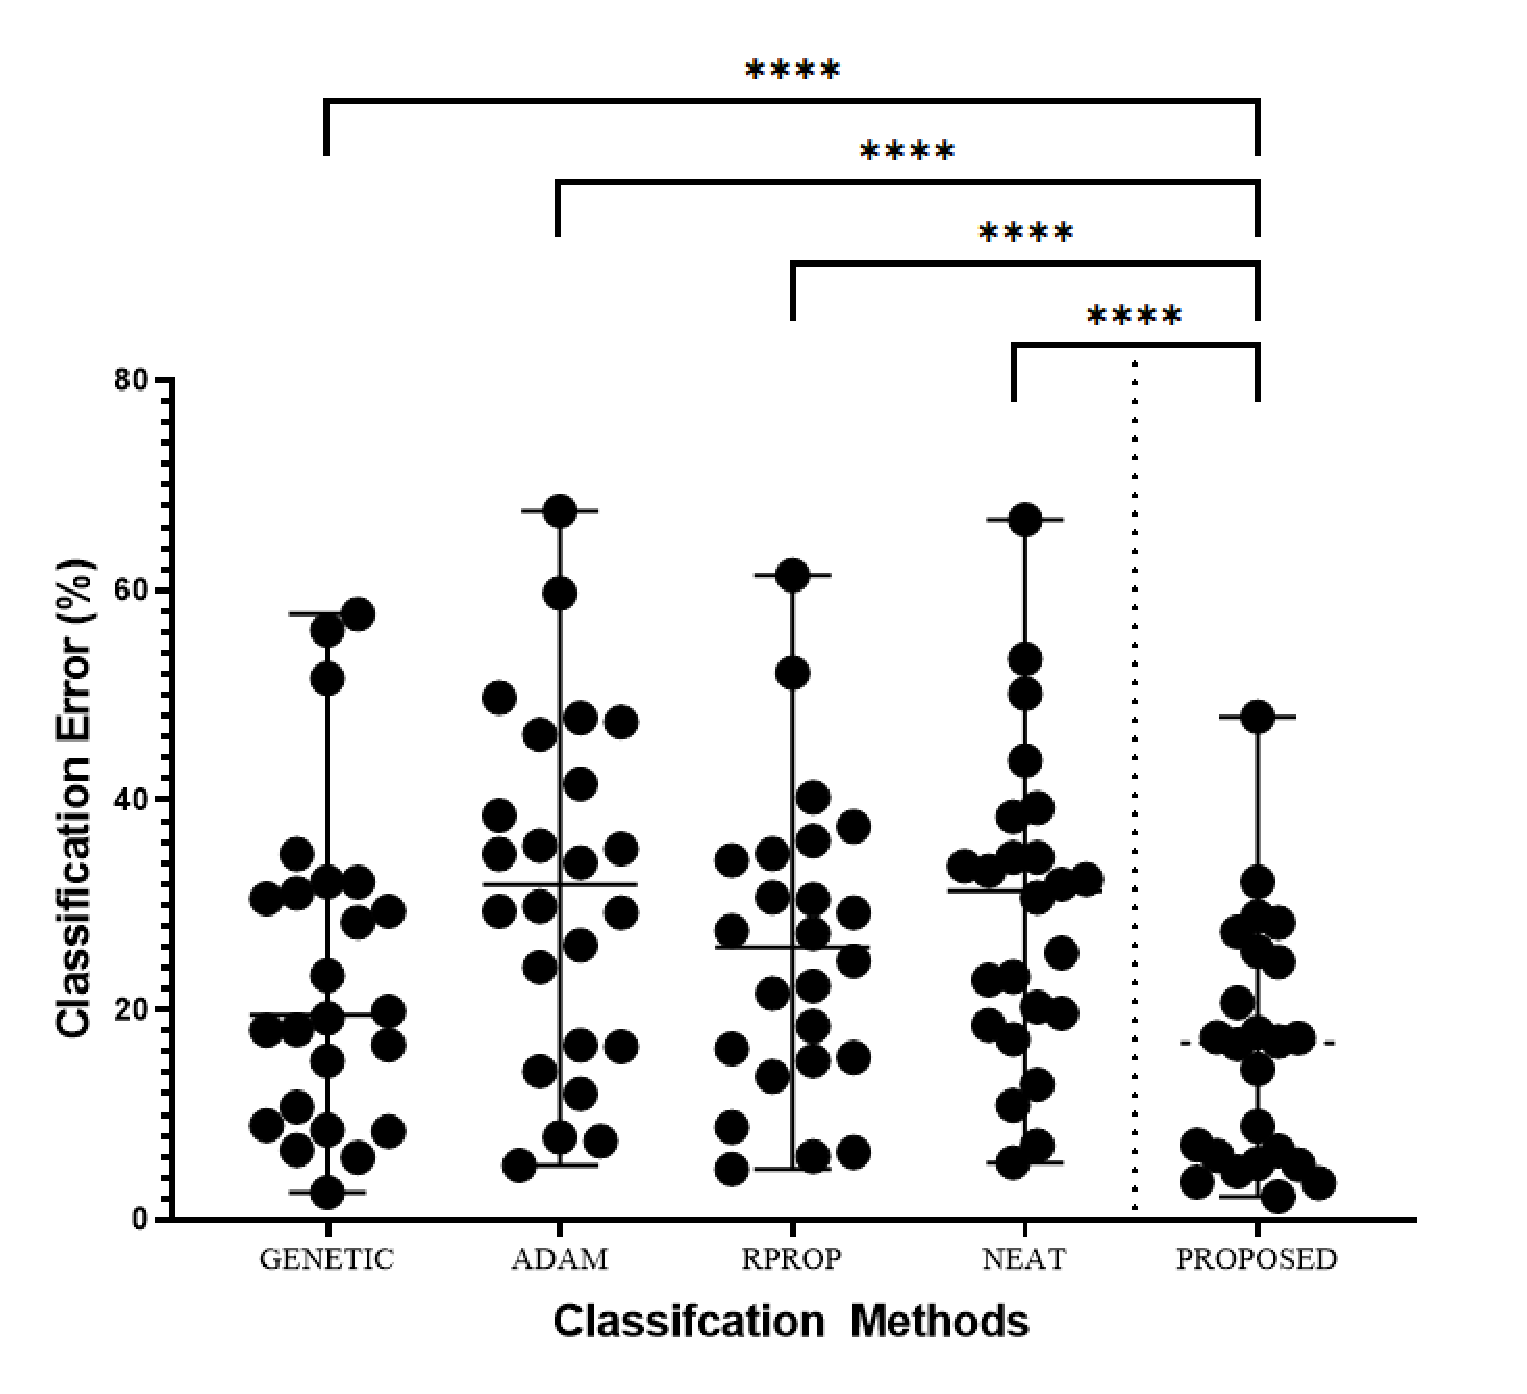
\includegraphics[scale=0.5]{class_grammar_neural}
\par\end{centering}
\caption{Scatter plot representation and the two-sample paired (Wilcoxon) signed-rank
test results of the comparison for each of the four (4) classification
methods (GENETIC, ADAM, RPROP, and NEAT) with the PROPOSED method
regarding the classification error in twenty-four (24) different public
available classification datasets. The stars only intend to flag significance
levels for the two most used groups. A p-value of less than 0.0001
is flagged with four stars ({*}{*}{*}{*}).\label{fig:ScatterClass}}

\end{figure}
\begin{figure}[H]
\begin{centering}
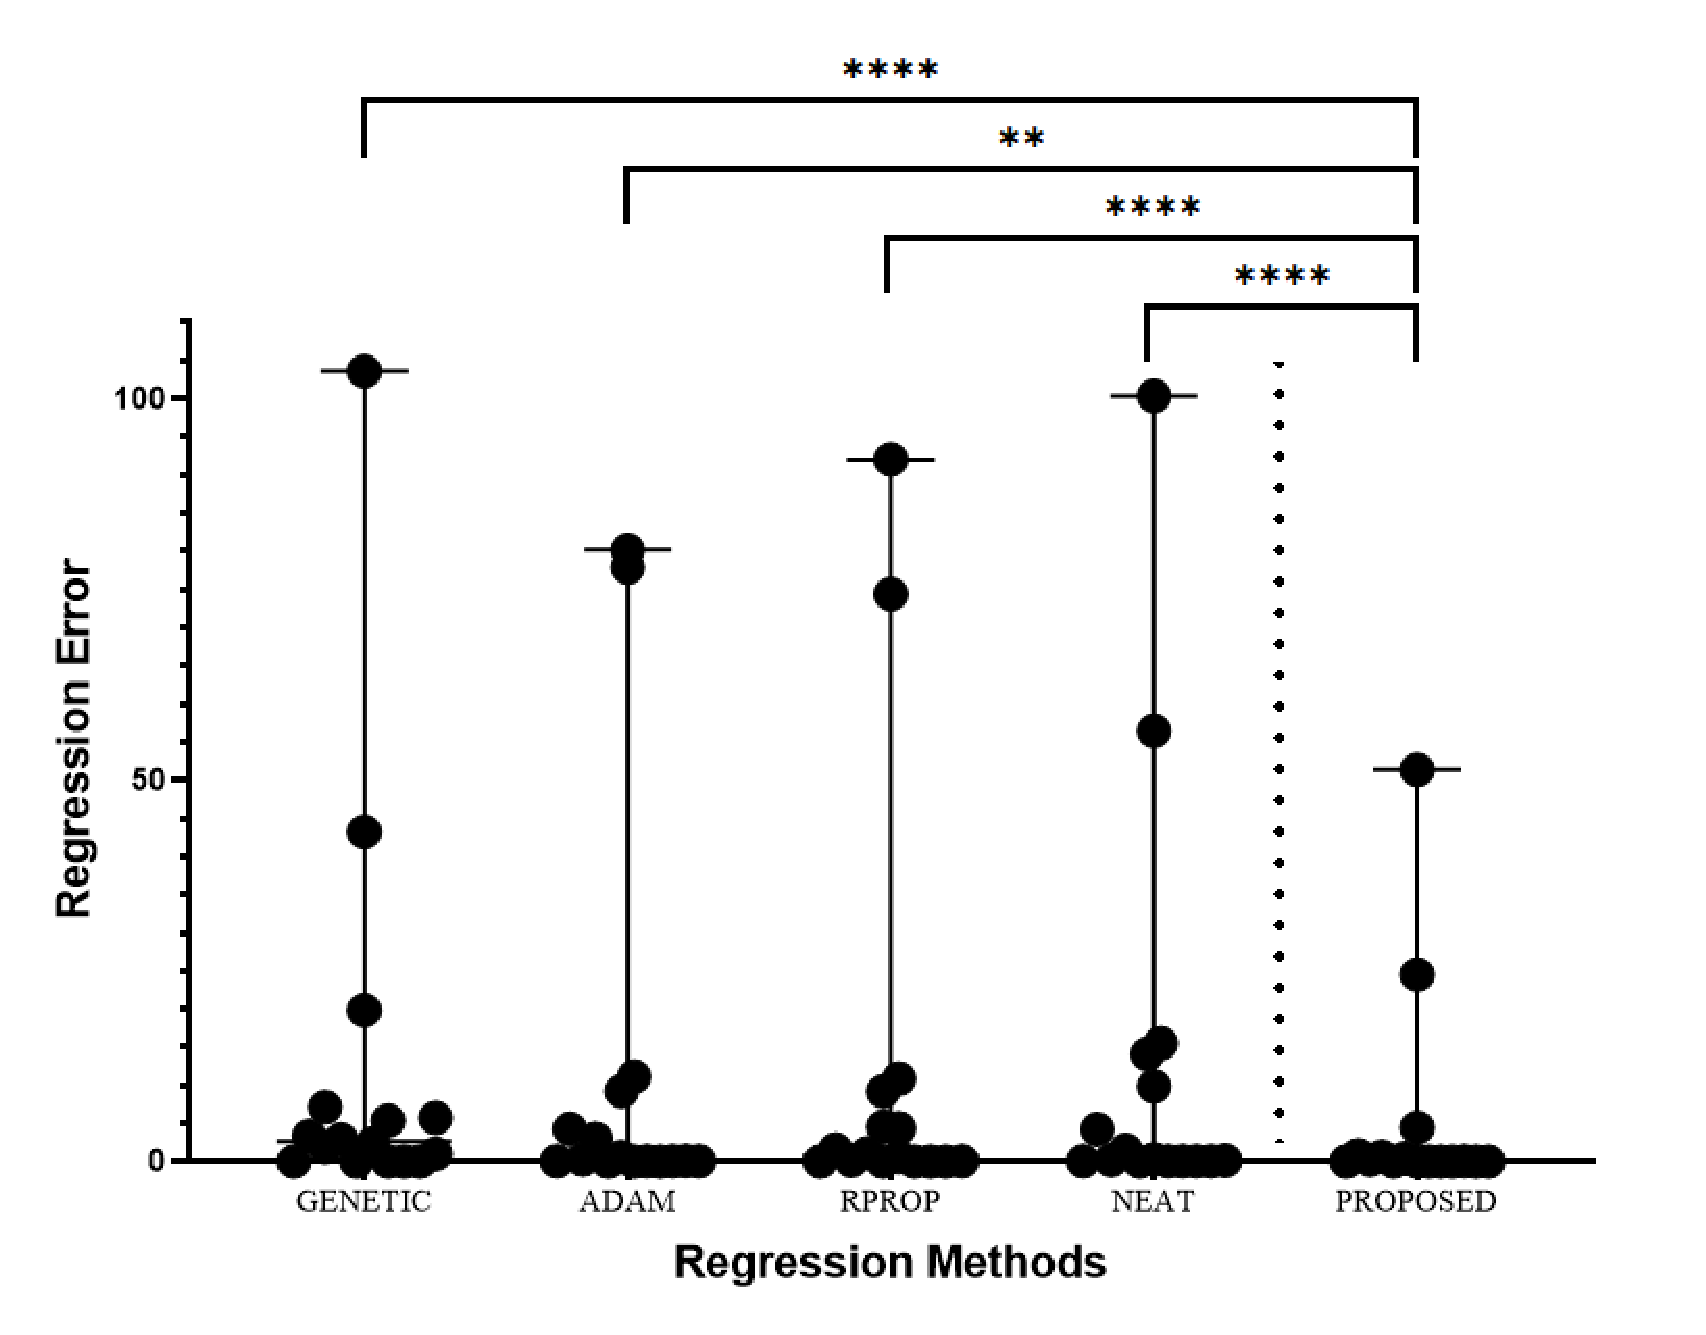
\includegraphics[scale=0.5]{regression_grammar_neural}
\par\end{centering}
\caption{Scatter plot representation and the Wilcoxon signed-rank test results
of the comparison for each of the four (4) regression methods (GENETIC,
ADAM, RPROP, and NEAT) with the PROPOSED method regarding the regression
error in sixteen (16) different publicly available regression datasets.
Star links join significantly different values; one star ({*}) stands
for p\textless 0.001, and four stars ({*}{*}{*} ) stand for p\textless 0.0001.
\label{fig:ScatterRegression}}

\end{figure}


\section{Conclusions \label{sec:Conclusions}}

This paper proposed a two-step technique to efficiently find a reliable
interval of values for the parameters of artificial neural networks.
In the first stage with partitioning techniques and using Grammatical
Evolution, a range of parameter values was searched and, in the second
stage, a genetic algorithm trained the artificial neural network within
the optimal range of values of the first stage. The proposed technique
is highly general and has been successfully applied to both data fitting
and classification problems. In both cases, the experimental results
demonstrate its superiority over other techniques appearing in the
relevant literature on the training of artificial neural networks.
In fact, in many cases in the performed experiments, the proposed
method outperforms others that were tested in percentages that exceed
70\%. In the future, a series of actions can be carried out to improve
the results and speed up the proposed method, such as:
\begin{enumerate}
\item There is a need for more efficient techniques for initializing the
value space for artificial neural network parameters. In the present
work, the optimal result from the execution of a limited number of
steps by a genetic algorithm was used as an initial estimate of the
value interval.
\item In the present work, the same techniques as in any whole-chromosome
genetic algorithm were used to perform the crossover and mutation
operations. Research could be done at this point to find more focused
crossover and mutation techniques for this particular problem.
\item The present technique consists of two phases, in each of which a problem-adapted
genetic algorithm is executed. This means that significant computational
time is required to complete the algorithm. However, since genetic
algorithms are inherently parallelizable, modern parallel programming
techniques could be used here.
\end{enumerate}
\vspace{6pt}


\authorcontributions{I.G.T., A.T. and E.K. conceived the idea and methodology and supervised
the technical part regarding the software. I.G.T. conducted the experiments,
employing several datasets, and provided the comparative experiments.
A.T. performed the statistical analysis. E.K. and all other authors
prepared the manuscript. E.K. and I.G.T. organized the research team
and A.T. supervised the project. All authors have read and agreed
to the published version of the manuscript.}

\funding{This research received no external funding.}

\institutionalreview{Not applicable.}

\informedconsent{Not applicable. }

\informedconsent{Not applicable. }

\acknowledgments{This research has been financed by the European Union : Next Generation
EU through the Program Greece 2.0 National Recovery and Resilience
Plan , under the call RESEARCH -- CREATE -- INNOVATE, project name
“iCREW: Intelligent small craft simulator for advanced crew training
using Virtual Reality techniques\textquotedbl{} (project code:TAEDK-06195
\quad{}}

\conflictsofinterest{The authors declare no conflict of interest.}

\sampleavailability{Not applicable.}

\appendixtitles{no}

\appendixstart{}

\appendix

\begin{adjustwidth}{-\extralength}{0cm}{}


\reftitle{References}
\begin{thebibliography}{99}
\bibitem{nn1}C. Bishop, Neural Networks for Pattern Recognition,
Oxford University Press, 1995.

\bibitem{nn2}G. Cybenko, Approximation by superpositions of a sigmoidal
function, Mathematics of Control Signals and Systems \textbf{2}, pp.
303-314, 1989.

\bibitem{nnphysics1}P. Baldi, K. Cranmer, T. Faucett et al, Parameterized
neural networks for high-energy physics, Eur. Phys. J. C \textbf{76},
2016.

\bibitem{nnphysics2}J. J. Valdas and G. Bonham-Carter, Time dependent
neural network models for detecting changes of state in complex processes:
Applications in earth sciences and astronomy, Neural Networks \textbf{19},
pp. 196-207, 2006

\bibitem{nnphysics3}G. Carleo,M. Troyer, Solving the quantum many-body
problem with artificial neural networks, Science \textbf{355}, pp.
602-606, 2017.

\bibitem{nnde1}Y. Shirvany, M. Hayati, R. Moradian, Multilayer perceptron
neural networks with novel unsupervised training method for numerical
solution of the partial differential equations, Applied Soft Computing
\textbf{9}, pp. 20-29, 2009.

\bibitem{nnde2}A. Malek, R. Shekari Beidokhti, Numerical solution
for high order differential equations using a hybrid neural network---Optimization
method, Applied Mathematics and Computation \textbf{183}, pp. 260-271,
2006.

\bibitem{nnagr1}A. Topuz, Predicting moisture content of agricultural
products using artificial neural networks, Advances in Engineering
Software \textbf{41}, pp. 464-470, 2010.

\bibitem{nnagr2}A. Escamilla-García, G.M. Soto-Zarazúa, M. Toledano-Ayala,
E. Rivas-Araiza, A. Gastélum-Barrios, Abraham,Applications of Artificial
Neural Networks in Greenhouse Technology and Overview for Smart Agriculture
Development, Applied Sciences \textbf{10}, Article number 3835, 2020.

\bibitem{nnchem1}Lin Shen, Jingheng Wu, and Weitao Yang, Multiscale
Quantum Mechanics/Molecular Mechanics Simulations with Neural Networks,
Journal of Chemical Theory and Computation \textbf{12}, pp. 4934-4946,
2016.

\bibitem{nnchem2}Sergei Manzhos, Richard Dawes, Tucker Carrington,
Neural network‐based approaches for building high dimensional and
quantum dynamics‐friendly potential energy surfaces, Int. J. Quantum
Chem. \textbf{115}, pp. 1012-1020, 2015.

\bibitem{nnchem3}Jennifer N. Wei, David Duvenaud, and Alán Aspuru-Guzik,
Neural Networks for the Prediction of Organic Chemistry Reactions,
ACS Central Science \textbf{2}, pp. 725-732, 2016.

\bibitem{nnecon1}Lukas Falat and Lucia Pancikova, Quantitative Modelling
in Economics with Advanced Artificial Neural Networks, Procedia Economics
and Finance \textbf{34}, pp. 194-201, 2015.

\bibitem{nnecon2}Mohammad Namazi, Ahmad Shokrolahi, Mohammad Sadeghzadeh
Maharluie, Detecting and ranking cash flow risk factors via artificial
neural networks technique, Journal of Business Research \textbf{69},
pp. 1801-1806, 2016.

\bibitem{nncecon3}G. Tkacz, Neural network forecasting of Canadian
GDP growth, International Journal of Forecasting \textbf{17}, pp.
57-69, 2001.

\bibitem{nnmed1}Igor I. Baskin, David Winkler and Igor V. Tetko,
A renaissance of neural networks in drug discovery, Expert Opinion
on Drug Discovery \textbf{11}, pp. 785-795, 2016.

\bibitem{nnmed2}Ronadl Bartzatt, Prediction of Novel Anti-Ebola Virus
Compounds Utilizing Artificial Neural Network (ANN), Chemistry Faculty
Publications \textbf{49}, pp. 16-34, 2018.

\bibitem{nnc}I.G. Tsoulos, D. Gavrilis, E. Glavas, Neural network
construction and training using grammatical evolution, Neurocomputing
\textbf{72}, pp. 269-277, 2008.

\bibitem{bpnn}D.E. Rumelhart, G.E. Hinton and R.J. Williams, Learning
representations by back-propagating errors, Nature \textbf{323}, pp.
533 - 536 , 1986.

\bibitem{bpnn2}T. Chen and S. Zhong, Privacy-Preserving Backpropagation
Neural Network Learning, IEEE Transactions on Neural Networks \textbf{20},
, pp. 1554-1564, 2009.

\bibitem{rpropnn-1}M. Riedmiller and H. Braun, A Direct Adaptive
Method for Faster Backpropagation Learning: The RPROP algorithm, Proc.
of the IEEE Intl. Conf. on Neural Networks, San Francisco, CA, pp.
586--591, 1993.

\bibitem{rpropnn3}T. Pajchrowski, K. Zawirski and K. Nowopolski,
Neural Speed Controller Trained Online by Means of Modified RPROP
Algorithm, IEEE Transactions on Industrial Informatics \textbf{11},
pp. 560-568, 2015.

\bibitem{rpropnn2}Rinda Parama Satya Hermanto, Suharjito, Diana,
Ariadi Nugroho, Waiting-Time Estimation in Bank Customer Queues using
RPROP Neural Networks, Procedia Computer Science \textbf{ 135}, pp.
35-42, 2018.

\bibitem{Adam}D. P. Kingma, J. L. Ba, ADAM: a method for stochastic
optimization, in: Proceedings of the 3rd International Conference
on Learning Representations (ICLR 2015), pp. 1--15, 2015.

\bibitem{AdamNN}Y. Xue, Y. Tong, F. Neri, An ensemble of differential
evolution and Adam for training feed-forward neural networks. Information
Sciences \textbf{608}, pp. 453-471, 2022.

\bibitem{quasinn}B. Robitaille and B. Marcos and M. Veillette and
G. Payre, Modified quasi-Newton methods for training neural networks,
Computers \& Chemical Engineering \textbf{20}, pp. 1133-1140, 1996.

\bibitem{quasinn2}Q. Liu, J. Liu, R. Sang, J. Li, T. Zhang and Q.
Zhang, Fast Neural Network Training on FPGA Using Quasi-Newton Optimization
Method,IEEE Transactions on Very Large Scale Integration (VLSI) Systems
\textbf{26}, pp. 1575-1579, 2018.

\bibitem{tabunn}R.S. Sexton, B. Alidaee, R.E. Dorsey, J.D. Johnson,
Global optimization for artificial neural networks: A tabu search
application. European Journal of Operational Research \textbf{106},
pp. 570-584, 1998.

\bibitem{nn_ann1}A. Yamazaki, M. C. P. de Souto,T. B. Ludermir, Optimization
of neural network weights and architectures for odor recognition using
simulated annealing, In: Proceedings of the 2002 International Joint
Conference on Neural Networks. IJCNN'02 \textbf{1}, pp. 547-552 ,
2002.

\bibitem{nn_ann2}Y. Da, G. Xiurun, An improved PSO-based ANN with
simulated annealing technique, Neurocomputing \textbf{63}, pp. 527-533,
2005.

\bibitem{geneticnn}F. H. F. Leung, H. K. Lam, S. H. Ling and P. K.
S. Tam, Tuning of the structure and parameters of a neural network
using an improved genetic algorithm, IEEE Transactions on Neural Networks
\textbf{14}, pp. 79-88, 2003

\bibitem{geneticnn2}X. Yao, Evolving artificial neural networks,
Proceedings of the IEEE, 87(9), pp. 1423-1447, 1999.

\bibitem{psonn}C. Zhang, H. Shao and Y. Li, Particle swarm optimisation
for evolving artificial neural network, IEEE International Conference
on Systems, Man, and Cybernetics, , pp. 2487-2490, 2000.

\bibitem{psonn2}Jianbo Yu, Shijin Wang, Lifeng Xi, Evolving artificial
neural networks using an improved PSO and DPSO \textbf{71}, pp. 1054-1060,
2008.

\bibitem{weight_de1}J. lonen, J.K. Kamarainen, J. Lampinen, Differential
Evolution Training Algorithm for Feed-Forward Neural Networks, Neural
Processing Letters \textbf{17}, pp. 93--105, 2003.

\bibitem{weight_de2}M. Baioletti, G. Di Bari, A. Milani, V. Poggioni,
Differential Evolution for Neural Networks Optimization, Mathematics
\textbf{8}, 2020.

\bibitem{weight_aco}K.M. Salama, A.M. Abdelbar, Learning neural network
structures with ant colony algorithms, Swarm Intell \textbf{9}, pp.
229--265, 2015.

\bibitem{nnhybrid1}J.R. Zhang, J. Zhang, T.M. Lok, M.R. Lyu, A hybrid
particle swarm optimization--back-propagation algorithm for feedforward
neural network training, Applied Mathematics and Computation \textbf{185},
pp. 1026-1037, 2007.

\bibitem{nnhybrid2}S. Mishra, S. K. Patra, Short Term Load Forecasting
Using Neural Network Trained with Genetic Algorithm \& Particle Swarm
Optimization, In: 2008 First International Conference on Emerging
Trends in Engineering and Technology, Nagpur, India, 2008, pp. 606-611,
doi: 10.1109/ICETET.2008.94.

\bibitem{nnhybrid3}S. Mirjalili, S.Z. Mohd Hashim, H. Moradian Sardroudi,
Training feedforward neural networks using hybrid particle swarm optimization
and gravitational search algorithm, Applied Mathematics and Computation
\textbf{218}, pp. 11125-11137, 2012.

\bibitem{nnhybrid4}A. Kobrunov, I. Priezzhev, Hybrid combination
genetic algorithm and controlled gradient method to train a neural
network, Geophysics \textbf{81}, pp,35--43, 2016. 

\bibitem{weight_init1}I. Ivanova, M. Kubat, Initialization of neural
networks by means of decision trees, Knowledge-Based Systems \textbf{8},
pp. 333-344, 1995.

\bibitem{weight_init2}J.Y.F. Yam, T.W.S. Chow, A weight initialization
method for improving training speed in feedforward neural network,
Neurocomputing \textbf{30}, pp. 219-232, 2000.

\bibitem{weight_init3}K. Chumachenko, A. Iosifidis, M. Gabbouj, Feedforward
neural networks initialization based on discriminant learning, Neural
Networks \textbf{146}, pp. 220-229, 2022.

\bibitem{weight_decay1}M.D. Shahjahan, M. Kazuyuki, Neural network
training algorithm with possitive correlation, IEEE Trans. Inf \&
Syst. \textbf{88}, pp. 2399-2409, 2005.

\bibitem{weight_decay2}N.K. Treadgold, T.D. Gedeon, Simulated annealing
and weight decay in adaptive learning: the SARPROP algorithm, IEEE
Trans. on Neural Networks \textbf{9}, pp. 662-668, 1998.

\bibitem{weight_decay3}C.S. Leung, K.W. Wong, P.F. Sum, L.W. Chan,
A pruning method for the recursive least squared algorithm, Neural
networks \textbf{14}, pp. 147-174, 2001.

\bibitem{ge1}M. O’Neill, C. Ryan, Grammatical evolution, IEEE Trans.
Evol. Comput. \textbf{5,}pp. 349--358, 2001.

\bibitem{bnf1}J. W. Backus. The Syntax and Semantics of the Proposed
International Algebraic Language of the Zurich ACM-GAMM Conference.
Proceedings of the International Conference on Information Processing,
UNESCO, 1959, pp.125-132.

\bibitem{ge_program1}C. Ryan, J. Collins, M. O’Neill, Grammatical
evolution: Evolving programs for an arbitrary language. In: Banzhaf,
W., Poli, R., Schoenauer, M., Fogarty, T.C. (eds) Genetic Programming.
EuroGP 1998. Lecture Notes in Computer Science, vol 1391. Springer,
Berlin, Heidelberg, 1998.

\bibitem{ge_program2}M. O’Neill, M., C. Ryan, Evolving Multi-line
Compilable C Programs. In: Poli, R., Nordin, P., Langdon, W.B., Fogarty,
T.C. (eds) Genetic Programming. EuroGP 1999. Lecture Notes in Computer
Science, vol 1598. Springer, Berlin, Heidelberg, 1999.

\bibitem{ge_trig}C. Ryan, M. O’Neill, J.J. Collins, Grammatical evolution:
Solving trigonometric identities, proceedings of Mendel. Vol. 98.
1998.

\bibitem{ge_music}A.O. Puente, R. S. Alfonso, M. A. Moreno, Automatic
composition of music by means of grammatical evolution, In: APL '02:
Proceedings of the 2002 conference on APL: array processing languages:
lore, problems, and applications July 2002 Pages 148--155. 

\bibitem{ge_nn}Lídio Mauro Limade Campo, R. Célio Limã Oliveira,Mauro
Roisenberg, Optimization of neural networks through grammatical evolution
and a genetic algorithm, Expert Systems with Applications \textbf{56},
pp. 368-384, 2016.

\bibitem{ge_nn2}K. Soltanian, A. Ebnenasir, M. Afsharchi, Modular
Grammatical Evolution for the Generation of Artificial Neural Networks,
Evolutionary Computation \textbf{30}, pp 291--327, 2022.

\bibitem{ge_constant}I. Dempsey, M.O' Neill, A. Brabazon, Constant
creation in grammatical evolution, International Journal of Innovative
Computing and Applications \textbf{1} , pp 23--38, 2007.

\bibitem{ge_pacman}E. Galván-López, J.M. Swafford, M. O’Neill, A.
Brabazon, Evolving a Ms. PacMan Controller Using Grammatical Evolution.
In: , et al. Applications of Evolutionary Computation. EvoApplications
2010. Lecture Notes in Computer Science, vol 6024. Springer, Berlin,
Heidelberg, 2010.

\bibitem{ge_supermario}N. Shaker, M. Nicolau, G. N. Yannakakis, J.
Togelius, M. O'Neill, Evolving levels for Super Mario Bros using grammatical
evolution, 2012 IEEE Conference on Computational Intelligence and
Games (CIG), 2012, pp. 304-31.

\bibitem{ge_energy}D. Martínez-Rodríguez, J. M. Colmenar, J. I. Hidalgo,
R.J. Villanueva Micó, S. Salcedo-Sanz, Particle swarm grammatical
evolution for energy demand estimation, Energy Science and Engineering
\textbf{8}, pp. 1068-1079, 2020.

\bibitem{ge_comb}N. R. Sabar, M. Ayob, G. Kendall, R. Qu, Grammatical
Evolution Hyper-Heuristic for Combinatorial Optimization Problems,
IEEE Transactions on Evolutionary Computation \textbf{17}, pp. 840-861,
2013.

\bibitem{ge_crypt}C. Ryan, M. Kshirsagar, G. Vaidya, G. et al. Design
of a cryptographically secure pseudo random number generator with
grammatical evolution. Sci Rep \textbf{12}, 8602, 2022.

\bibitem{ge_decision}P.J. Pereira, P. Cortez, R. Mendes, Multi-objective
Grammatical Evolution of Decision Trees for Mobile Marketing user
conversion prediction, Expert Systems with Applications \textbf{168},
114287, 2021.

\bibitem{ge_analog}F. Castejón, E.J. Carmona, Automatic design of
analog electronic circuits using grammatical evolution, Applied Soft
Computing \textbf{62}, pp. 1003-1018, 2018.

\bibitem{kaelo}P. Kaelo, M.M. Ali, Integrated crossover rules in
real coded genetic algorithms, European Journal of Operational Research
\textbf{176}, pp. 60-76, 2007.

\bibitem{powell}M.J.D Powell, A Tolerant Algorithm for Linearly Constrained
Optimization Calculations, Mathematical Programming \textbf{45}, pp.
547-566, 1989. 

\bibitem{UCL}M. Kelly, R. Longjohn, K. Nottingham, The UCI Machine
Learning Repository. 2023. Available online: https://archive.ics.uci.edu
(accessed on 20 September 2023).

\bibitem{Keel}J. Alcalá-Fdez, A. Fernandez, J. Luengo, J. Derrac,
S. García, L. Sánchez, F. Herrera. KEEL Data-Mining Software Tool:
Data Set Repository, Integration of Algorithms and Experimental Analysis
Framework. Journal of Multiple-Valued Logic and Soft Computing 17,
pp. 255-287, 2011.

\bibitem{appendicitis}Weiss, Sholom M. and Kulikowski, Casimir A.,
Computer Systems That Learn: Classification and Prediction Methods
from Statistics, Neural Nets, Machine Learning, and Expert Systems,
Morgan Kaufmann Publishers Inc, 1991.

\bibitem{australian}J.R. Quinlan, Simplifying Decision Trees. International
Journal of Man-Machine Studies \textbf{27}, pp. 221-234, 1987. 

\bibitem{balance}T. Shultz, D. Mareschal, W. Schmidt, Modeling Cognitive
Development on Balance Scale Phenomena, Machine Learning \textbf{16},
pp. 59-88, 1994.

\bibitem{cleveland1}Z.H. Zhou,Y. Jiang, NeC4.5: neural ensemble based
C4.5,\textquotedbl{} in IEEE Transactions on Knowledge and Data Engineering
\textbf{16}, pp. 770-773, 2004.

\bibitem{cleveland2}R. Setiono , W.K. Leow, FERNN: An Algorithm for
Fast Extraction of Rules from Neural Networks, Applied Intelligence
\textbf{12}, pp. 15-25, 2000.

\bibitem{dermatology}G. Demiroz, H.A. Govenir, N. Ilter, Learning
Differential Diagnosis of Eryhemato-Squamous Diseases using Voting
Feature Intervals, Artificial Intelligence in Medicine. \textbf{13},
pp. 147--165, 1998.

\bibitem{heart}I. Kononenko, E. Šimec, M. Robnik-Šikonja, Overcoming
the Myopia of Inductive Learning Algorithms with RELIEFF, Applied
Intelligence \textbf{7}, pp. 39--55, 1997

\bibitem{hayesroth}B. Hayes-Roth, B., F. Hayes-Roth. Concept learning
and the recognition and classification of exemplars. Journal of Verbal
Learning and Verbal Behavior \textbf{16}, pp. 321-338, 1977.

\bibitem{housevotes}R.M. French, N. Chater, Using noise to compute
error surfaces in connectionist networks: a novel means of reducing
catastrophic forgetting, Neural Comput. \textbf{14}, pp. 1755-1769,
2002.

\bibitem{ion1}J.G. Dy , C.E. Brodley, Feature Selection for Unsupervised
Learning, The Journal of Machine Learning Research \textbf{5}, pp
845--889, 2004.

\bibitem{ion2}S. J. Perantonis, V. Virvilis, Input Feature Extraction
for Multilayered Perceptrons Using Supervised Principal Component
Analysis, Neural Processing Letters \textbf{10}, pp 243--252, 1999.

\bibitem{liver} J. Garcke, M. Griebel, Classification with sparse
grids using simplicial basis functions, Intell. Data Anal. \textbf{6},
pp. 483-502, 2002.

\bibitem{mammographic}M. Elter, R. Schulz-Wendtland, T. Wittenberg,
The prediction of breast cancer biopsy outcomes using two CAD approaches
that both emphasize an intelligible decision process, Med Phys. \textbf{34},
pp. 4164-72, 2007.

\bibitem{parkinsons}M.A. Little, P.E. McSharry, E.J. Hunter, J. Spielman,
L.O. Ramig, Suitability of dysphonia measurements for telemonitoring
of Parkinson's disease. IEEE Trans Biomed Eng. \textbf{56}, pp. 1015-1022,
2009.

\bibitem{pima}J.W. Smith, J.E. Everhart, W.C. Dickson, W.C. Knowler,
R.S. Johannes, Using the ADAP learning algorithm to forecast the onset
of diabetes mellitus, In: Proceedings of the Symposium on Computer
Applications and Medical Care IEEE Computer Society Press, pp.261-265,
1988.

\bibitem{popfailures}D.D. Lucas, R. Klein, J. Tannahill, D. Ivanova,
S. Brandon, D. Domyancic, Y. Zhang, Failure analysis of parameter-induced
simulation crashes in climate models, Geoscientific Model Development
\textbf{6}, pp. 1157-1171, 2013.

\bibitem{regions}N. Giannakeas, M.G. Tsipouras, A.T. Tzallas, K.
Kyriakidi, Z.E. Tsianou, P. Manousou, A. Hall, E.C. Karvounis, V.
Tsianos, E. Tsianos, A clustering based method for collagen proportional
area extraction in liver biopsy images (2015) Proceedings of the Annual
International Conference of the IEEE Engineering in Medicine and Biology
Society, EMBS, 2015-November, art. no. 7319047, pp. 3097-3100. 

\bibitem{saheart}T. Hastie, R. Tibshirani, Non-parametric logistic
and proportional odds regression, JRSS-C (Applied Statistics) \textbf{36},
pp. 260--276, 1987.

\bibitem{segment}M. Dash, H. Liu, P. Scheuermann, K. L. Tan, Fast
hierarchical clustering and its validation, Data \& Knowledge Engineering
\textbf{44}, pp 109--138, 2003.

\bibitem{wdbc}W.H. Wolberg, O.L. Mangasarian, Multisurface method
of pattern separation for medical diagnosis applied to breast cytology,
Proc Natl Acad Sci U S A. \textbf{87}, pp. 9193--9196, 1990.

\bibitem{wine1}M. Raymer, T.E. Doom, L.A. Kuhn, W.F. Punch, Knowledge
discovery in medical and biological datasets using a hybrid Bayes
classifier/evolutionary algorithm. IEEE transactions on systems, man,
and cybernetics. Part B, Cybernetics : a publication of the IEEE Systems,
Man, and Cybernetics Society, \textbf{33} , pp. 802-813, 2003.

\bibitem{wine2}P. Zhong, M. Fukushima, Regularized nonsmooth Newton
method for multi-class support vector machines, Optimization Methods
and Software \textbf{22}, pp. 225-236, 2007.

\bibitem{eeg}R.G. Andrzejak, K. Lehnertz, F. Mormann, C. Rieke, P.
David, and C. E. Elger, Indications of nonlinear deterministic and
finite-dimensional structures in time series of brain electrical activity:
Dependence on recording region and brain state, Phys. Rev. E \textbf{64},
pp. 1-8, 2001.

\bibitem{zoo}M. Koivisto, K. Sood, Exact Bayesian Structure Discovery
in Bayesian Networks, The Journal of Machine Learning Research\textbf{
5}, pp. 549--573, 2004.

\bibitem{key-20}R.G. Andrzejak, K. Lehnertz, F. Mormann, C. Rieke,
P. David, and C. E. Elger, Indications of nonlinear deterministic
and finite-dimensional structures in time series of brain electrical
activity: Dependence on recording region and brain state, Phys. Rev.
E \textbf{64}, pp. 1-8, 2001.

\bibitem{abalone}W. J Nash, T.L. Sellers, S.R. Talbot, A.J. Cawthor,
W.B. Ford, The Population Biology of Abalone (\_Haliotis\_ species)
in Tasmania. I. Blacklip Abalone (\_H. rubra\_) from the North Coast
and Islands of Bass Strait, Sea Fisheries Division, Technical Report
No. 48 (ISSN 1034-3288), 1994.

\bibitem{airfoil}T.F. Brooks, D.S. Pope, A.M. Marcolini, Airfoil
self-noise and prediction. Technical report, NASA RP-1218, July 1989. 

\bibitem{Stat}J.S. Simonoff, Smooting Methods in Statistics, Springer
- Verlag, 1996.

\bibitem{concrete}I.Cheng Yeh, Modeling of strength of high performance
concrete using artificial neural networks, Cement and Concrete Research.
\textbf{28}, pp. 1797-1808, 1998. 

\bibitem{key23}D. Harrison and D.L. Rubinfeld, Hedonic prices and
the demand for clean ai, J. Environ. Economics \& Management \textbf{5},
pp. 81-102, 1978.

\bibitem{key21}J.S. Simonoff, Smooting Methods in Statistics, Springer
- Verlag, 1996.

\bibitem{pydataset}R.D. King, S. Muggleton, R. Lewis, M.J.E. Sternberg,
Proc. Nat. Acad. Sci. USA \textbf{89}, pp. 11322--11326, 1992. 

\bibitem{neat}K. O. Stanley, R. Miikkulainen, Evolving Neural Networks
through Augmenting Topologies, Evolutionary Computation \textbf{10},
pp. 99-127, 2002.

\bibitem{genpar1}E. Cantu-Paz, D.E. Goldberg, Efficient parallel
genetic algorithms: theory and practice, Computer methods in applied
mechanics and engineering \textbf{186}, pp. 221-238, 2000.

\bibitem{genpar2}T. Harada, E. Alba, Parallel genetic algorithms:
a useful survey, ACM Computing Surveys (CSUR) \textbf{53}, pp. 1-39,
2022.

\bibitem{openmpi}W. Gropp, E. Lusk, N. Doss, A. Skjellum, A high-performance,
portable implementation of the MPI message passing interface standard,
Parallel Computing \textbf{22}, pp. 789-828, 1996.

\bibitem{openmp}R. Chandra, L. Dagum, D. Kohr, D. Maydan,J. McDonald
and R. Menon, Parallel Programming in OpenMP, Morgan Kaufmann Publishers
Inc., 2001.

\end{thebibliography}
%%%%%%%%%%%%%%%%%%%%%%%%%%%%%%%%%%%%%%%%%%
%% for journal Sci
%\reviewreports{\\
%Reviewer 1 comments and authors' response\\
%Reviewer 2 comments and authors' response\\
%Reviewer 3 comments and authors' response
%}
%%%%%%%%%%%%%%%%%%%%%%%%%%%%%%%%%%%%%%%%%%

\PublishersNote{}

\end{adjustwidth}{}
\end{document}
